\documentclass{article}

\usepackage{amsmath}
\usepackage{geometry}
\usepackage{graphicx}

\usepackage[utf8]{inputenc}
\usepackage{fourier} 
\usepackage{array}
\usepackage{makecell}

\renewcommand\theadalign{bc}
\renewcommand\theadfont{\bfseries}
\renewcommand\theadgape{\Gape[4pt]}
\renewcommand\cellgape{\Gape[4pt]}

\geometry{letterpaper, left=1cm, right=1cm, top=1.5cm, bottom=2cm}

\title{Adversarial Images}
\author{Adam Spindler}

\begin{document}
\maketitle

\section{Adversarial Examples by Random Perturbation}

The goal is to create adversarial images for a black box object detector. With no access to the model, a simple approach is to distort the source images in various ways with the hope that the model will no longer be able to see the objects in the images. Experiments were run to determine the effectiveness of this naive approach.

\subsection{Adding Noise}
Noise was added to the images by generating a random tensor the same size as the input image. The random tensor's values are between 0 and 1, and the image's pixel values are between 0 and 255. To adjust the noisiness of the images, the random tensor was multiplied by the integer parameter "noise" to scale it up. The noise multiplier used in each of the images is shown at the top of the column. The results of this experiment are visible in figure \ref{fig:randnoise}.

\begin{figure}[h]
\centering
\begin{tabular}{ c c c c }
    original & noise = 100 & noise = 200 & noise = 500 \\
    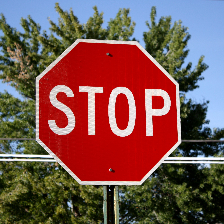
\includegraphics[width=0.2\linewidth]{../test_images/stop.png} & 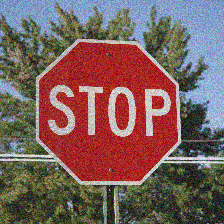
\includegraphics[width=0.2\linewidth]{../test_images/perturbed/stop_noise_100.png} & 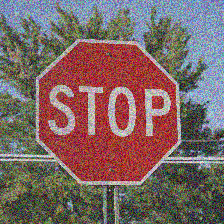
\includegraphics[width=0.2\linewidth]{../test_images/perturbed/stop_noise_200.png} & 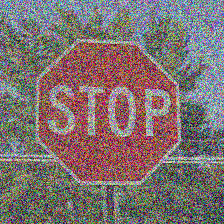
\includegraphics[width=0.2\linewidth]{../test_images/perturbed/stop_noise_500.png} \\
    \makecell{YOLOv3 = 0.99987 \\ RCNN = 0.99987} & \makecell{YOLOv3 = 0.99987 \\ RCNN = 0.99993} & \makecell{YOLOv3 = 0.99968 \\ RCNN = 0.99610} & \makecell{YOLOv3 = 0.99985 \\ RCNN = 0} \\[1cm]
    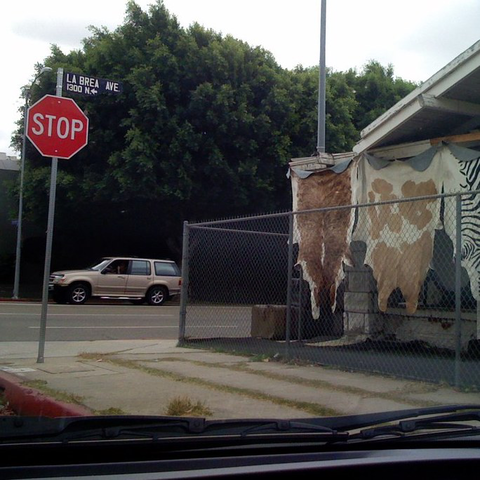
\includegraphics[width=0.2\linewidth]{../test_images/stop3.png} & 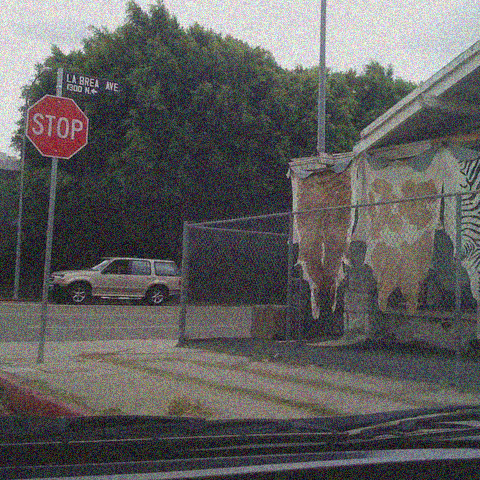
\includegraphics[width=0.2\linewidth]{../test_images/perturbed/stop3_noise_100.png} & 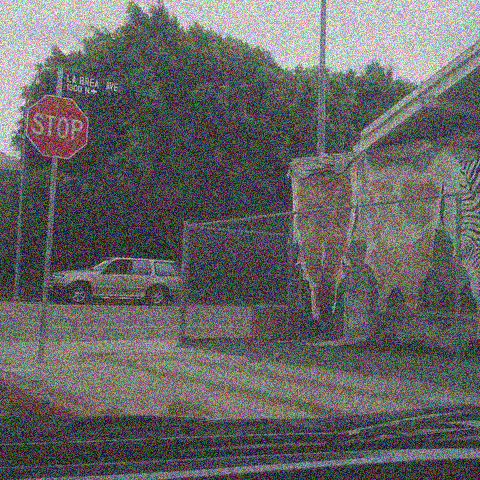
\includegraphics[width=0.2\linewidth]{../test_images/perturbed/stop3_noise_200.png} & 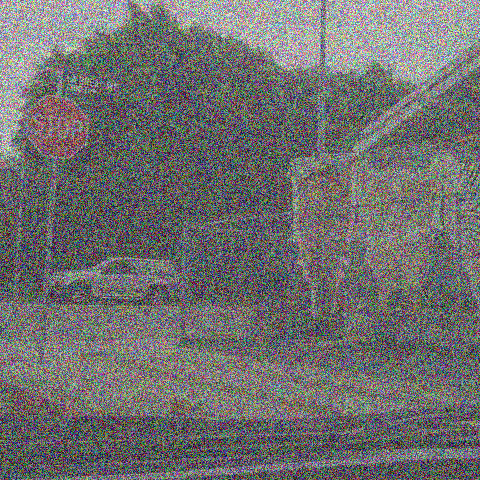
\includegraphics[width=0.2\linewidth]{../test_images/perturbed/stop3_noise_500.png} \\
    \makecell{YOLOv3 = 0.99971 \\ RCNN = 0.99839} & \makecell{YOLOv3 = 0.99995 \\ RCNN = 0.99926} & \makecell{YOLOv3 = 0.99951 \\ RCNN = 0.99850} & \makecell{YOLOv3 = 0 \\ RCNN = 0} \\  
\end{tabular}
\label{fig:randnoise}
\caption{Noise Experiment}
\end{figure}

\subsection{Grayscale}
The images were converted to grayscale by removing a percentage of their colors. The value used for each of the images is shown at the top of the columns. The results of this experiment are visible in figure \ref{fig:grayscale}.

\begin{figure}[h]
\centering
\begin{tabular}{ c c c c }
    original & color = 50\% & color = 25\% & color = 0\% \\
    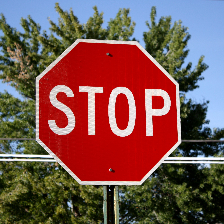
\includegraphics[width=0.2\linewidth]{../test_images/stop.png} & 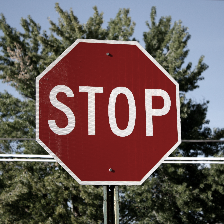
\includegraphics[width=0.2\linewidth]{../test_images/perturbed/stop_grayscale_0_500.png} & 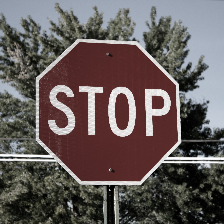
\includegraphics[width=0.2\linewidth]{../test_images/perturbed/stop_grayscale_0_250.png} & 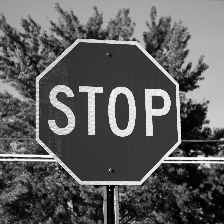
\includegraphics[width=0.2\linewidth]{../test_images/perturbed/stop_grayscale_0_010.png} \\
    \makecell{YOLOv3 = 0.99987 \\ RCNN = 0.99987} & \makecell{YOLOv3 = 0.99988 \\ RCNN = 0.99987} & \makecell{YOLOv3 = 0.99989 \\ RCNN = 0.99986} & \makecell{YOLOv3 = 0.99986 \\ RCNN = 0.99868} \\[1cm]
    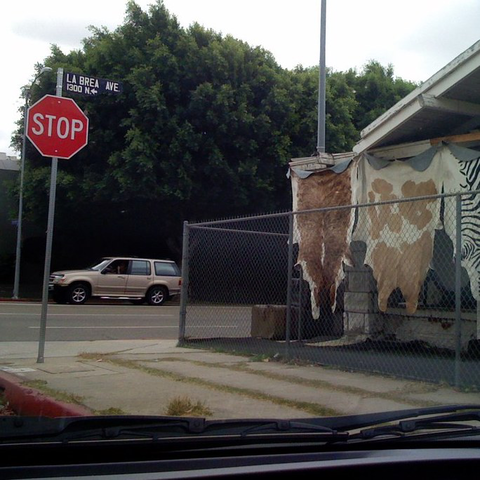
\includegraphics[width=0.2\linewidth]{../test_images/stop3.png} & 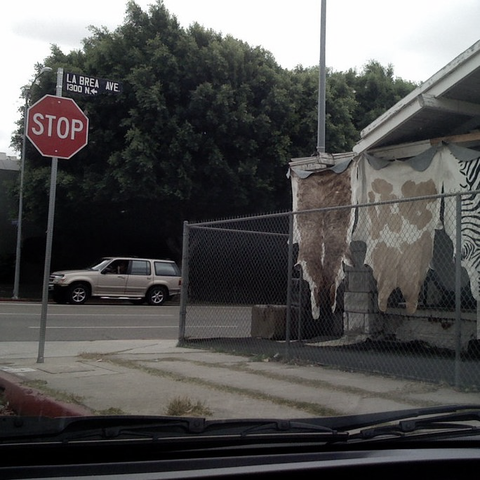
\includegraphics[width=0.2\linewidth]{../test_images/perturbed//stop3_grayscale_0_500.png} & 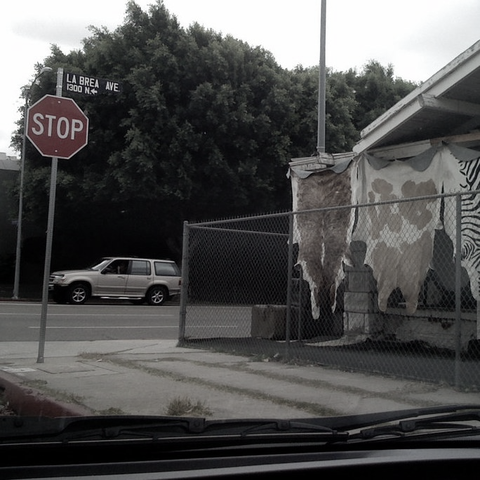
\includegraphics[width=0.2\linewidth]{../test_images/perturbed/stop3_grayscale_0_250.png} & 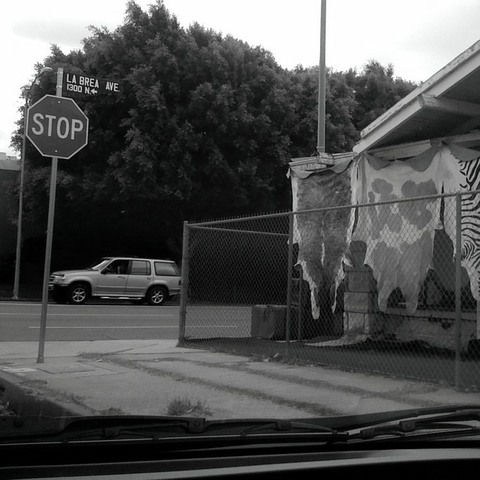
\includegraphics[width=0.2\linewidth]{../test_images/perturbed/stop3_grayscale_0_010.png} \\
    \makecell{YOLOv3 = 0.99971 \\ RCNN = 0.99839} & \makecell{YOLOv3 = 0.99971 \\ RCNN = 0.99859} & \makecell{YOLOv3 = 0.99970 \\ RCNN = 0.99866} & \makecell{YOLOv3 = 0.99965 \\ RCNN = 0.99846} \\  
\end{tabular}
\caption{Grayscale Experiment}
\label{fig:grayscale}
\end{figure}

\subsection{Contrast}
The contrast was adjusted for each of the images using the "Contrast" enhancer in Pillow's ImageEnhance package. The contrast parameter given to this enhancer is shown at the top of each column. The results of this experiment are visible in figure \ref{fig:contrast}.

\begin{figure}[h]
\centering
\begin{tabular}{ c c c c }
    original & contrast = 0.05 & contrast = 0.025 & contrast = 0.01 \\
    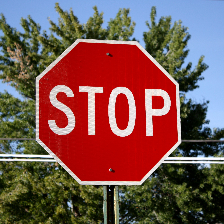
\includegraphics[width=0.2\linewidth]{../test_images/stop.png} & 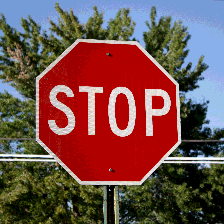
\includegraphics[width=0.2\linewidth]{../test_images/perturbed/stop_contrast_0_050.png} & 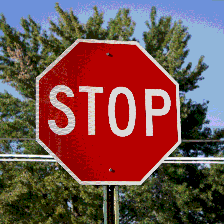
\includegraphics[width=0.2\linewidth]{../test_images/perturbed/stop_contrast_0_025.png} & 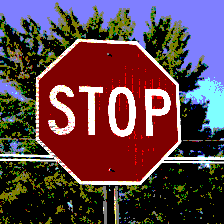
\includegraphics[width=0.2\linewidth]{../test_images/perturbed/stop_contrast_0_010.png} \\
    \makecell{YOLOv3 = 0.99987 \\ RCNN = 0.99987} & \makecell{YOLOv3 = 0.99985 \\ RCNN = 0.99994} & \makecell{YOLOv3 = 0.99986 \\ RCNN = 0.99993} & \makecell{YOLOv3 = 0.99984 \\ RCNN = 0.99859} \\[1cm]
    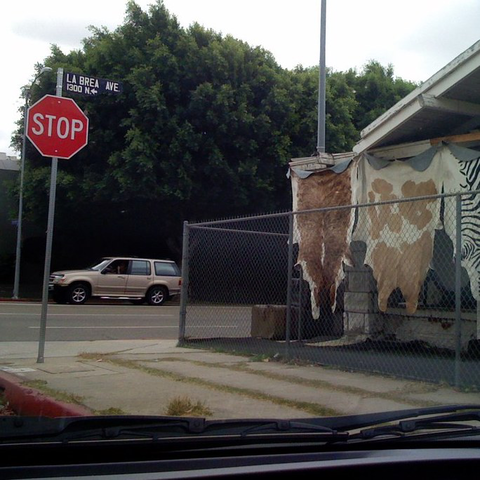
\includegraphics[width=0.2\linewidth]{../test_images/stop3.png} & 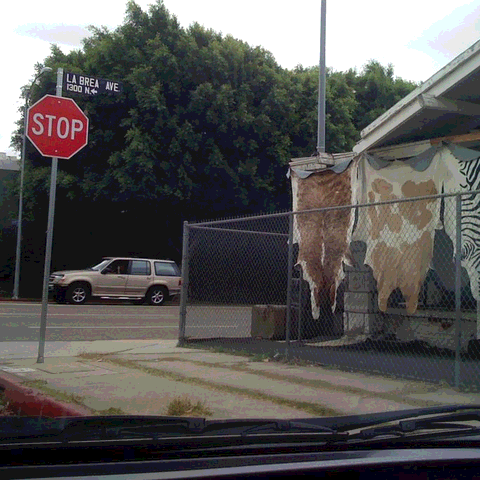
\includegraphics[width=0.2\linewidth]{../test_images/perturbed/stop3_contrast_0_050.png} & 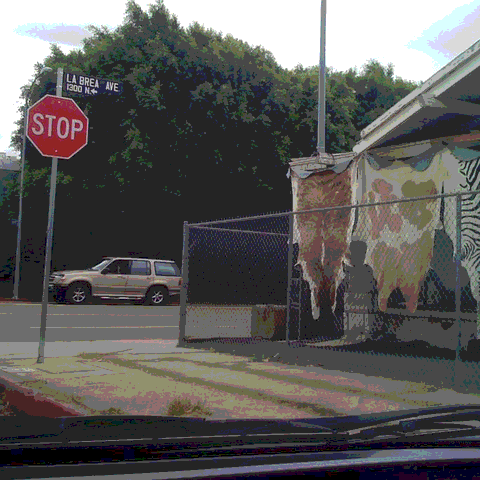
\includegraphics[width=0.2\linewidth]{../test_images/perturbed/stop3_contrast_0_025.png} & 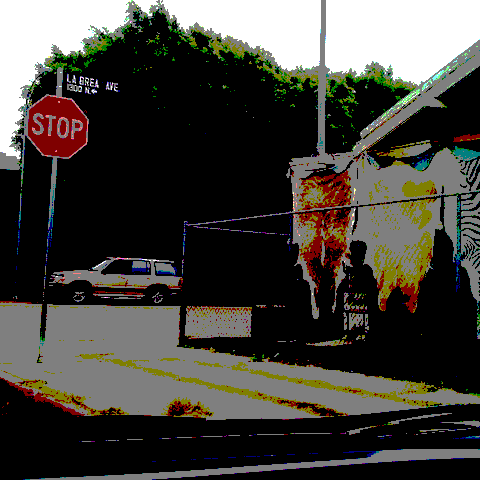
\includegraphics[width=0.2\linewidth]{../test_images/perturbed/stop3_contrast_0_010.png} \\
    \makecell{YOLOv3 = 0.99971 \\ RCNN = 0.99839} & \makecell{YOLOv3 = 0.99961 \\ RCNN = 0.99849} & \makecell{YOLOv3 = 0.99960 \\ RCNN = 0.99830} & \makecell{YOLOv3 = 0.99990 \\ RCNN = 0.99893} \\  
\end{tabular}
\caption{Contrast Experiment}
\label{fig:contrast}
\end{figure}

\subsection{Multiple Perturbations}
For these images all 3 perturbations were applied. First the contrast was set to 0.025, then noise was added with a multiplier of 200, and finally the color was removed from the image.

\begin{figure}[h]
\centering
\begin{tabular}{ c c }
    original & perturbed \\
    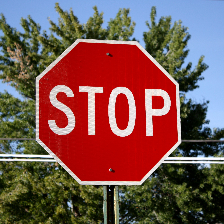
\includegraphics[width=0.3\linewidth]{../test_images/stop.png} & 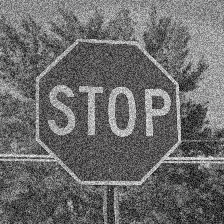
\includegraphics[width=0.3\linewidth]{../test_images/perturbed/stop_contrast_0_025_noise_200_grayscale_0_010.png} \\
    \makecell{YOLOv3 = 0.99987 \\ RCNN = 0.99987} & \makecell{YOLOv3 = 0.99992 \\ RCNN = 0} \\[1cm]
    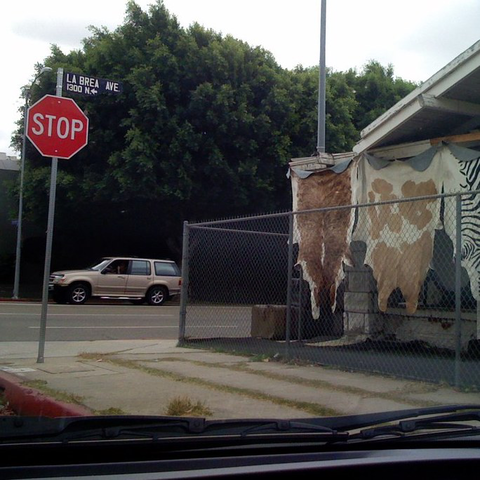
\includegraphics[width=0.3\linewidth]{../test_images/stop3.png} & 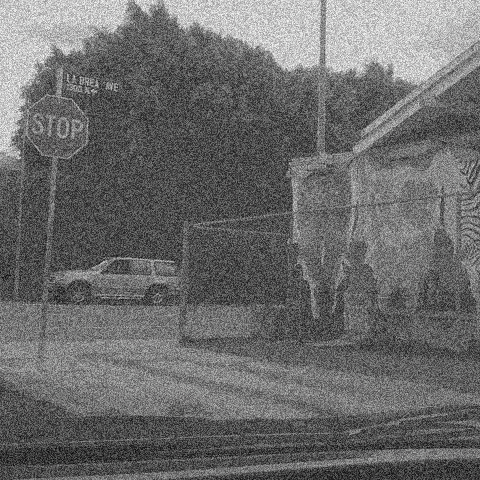
\includegraphics[width=0.3\linewidth]{../test_images/perturbed/stop3_contrast_0_025_noise_200_grayscale_0_010.png} \\
    \makecell{YOLOv3 = 0.99971 \\ RCNN = 0.99839} & \makecell{YOLOv3 = 0.99984 \\ RCNN = 0.99803} \\
\end{tabular}
\caption{Multiple Perturbation Experiment}
\label{fig:multiperturb}
\end{figure}

As shown in figure \ref{fig:multiperturb} random perturbation of images has little affect on the confidence score for both YOLOv3 and Faster-RCNN. The confidence score only drops when there is so much distortion that it is difficult to see what it is as a human.

Data augmentation is a popular technique used when training convolutional neural networks to increase the amount of data in the training set. Images are randomly modified in ways that do not change their label, such as translating the image, rotating it, adding random noise, and changing the colors \cite{shorten2019survey}. It is likely that both YOLOv3 and Faster-RCNN were trained using this technique which is why these perturbed images were mostly unsuccessful at fooling either of the models.

\section{Fast Gradient Sign Adversarial Images}

The fast gradient sign method for creating adversarial examples was first introduced by Goodfellow et al in \cite{goodfellow2015explaining}. This method works by computing the loss function for the input image, and then taking the derivative of the loss with respect to the input image. The sign of the gradient is then added to the input image to ascend the loss function and create as much misclassification error as possible.

\begin{equation}
    \eta = \epsilon * \text{sign} (\nabla_x L(x))
\end{equation}

Where $x$ is the input image, $L$ is the loss function which contains the classification model, $\epsilon$ is the learning rate, and $\eta$ is the perturbation to add to the input image.

The only problem with this method is that the output class that the model predicts after the perturbation is random, there isn't a way to choose it. A slight modification to the method was made so that instead of attempting to maximize the overall loss, the confidence score of a single class is used as the loss function to maximize. By optimizing this function, the confidence score of the target class will be increased.

\begin{equation}
    \eta = \epsilon * \text{sign} (\nabla_x (f_c(x))^2)
\end{equation}

Where $x$ is the input image and $f_c$ is the confidence score of the target class $c$ output by the model. This method was used to create adversarial examples on the VGG-16 \cite{simonyan2015deep} network, and run for several iterations of gradient descent until VGG-16 output the target class with a high confidence. In figure \ref{fig:vggadversarial} is a comparison between the input image and the adversarial image that was created. The last column shows the difference between the 2 images scaled up so the differences are visible. In the difference image the lighter pixels were changed the most, and the darker pixels were changed the least.

\begin{figure}[h]
\centering
\begin{tabular}{ c c c }
    original & adversarial & difference \\
    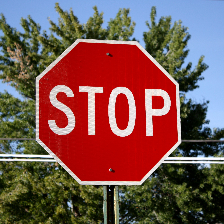
\includegraphics[width=0.3\linewidth]{../test_images/stop.png} & 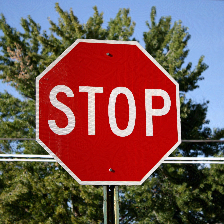
\includegraphics[width=0.3\linewidth]{../test_images/adversarial_vgg/stop.png} & 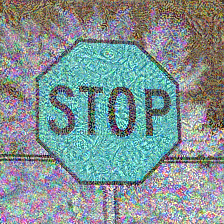
\includegraphics[width=0.3\linewidth]{../test_images/adversarial_vgg/stop_diff.png} \\
    \makecell{iPod confidence = 1.39 \\street sign confidence = 20.73} & \makecell{iPod confidence = 9.82 \\street sign confidence = 8.95} & \\
\end{tabular}
\caption{Adversarial Images for VGG-16}
\label{fig:vggadversarial}
\end{figure}

\section{Adversarial Examples Against YOLOv3}

Adversarial examples were created for YOLOv3 \cite{redmon2018yolov3} by using a technique similar to \cite{goodfellow2015explaining}. The output of YOLOv3 is a matrix, where each row is a possible bounding box prediction. The format of each row is as follows: 4 floats describing the bounding box, 1 float indicating the confidence score of an object actually being inside the bounding box, and 80 floats which are the confidence scores of each of the label classes.

The loss function made to create adversarial examples is the sum of all the bounding box confidence scores, and the confidence scores for the "stop sign" class. The loss function was regularized by adding the Euclidean distance between the adversarial image and the original image so the final adversarial image will have minimal visible changes, as described in \cite{szegedy2014intriguing}.

\begin{equation}
    \eta = \epsilon * [\nabla_{x} (g_{\text{bbox}}(f(x))) + g_{\text{stop}}(f(x)))] + (x - \hat{x})^2
\end{equation}

Where $\epsilon$ is the learning rate, $g_{\text{bbox}}$ is a function to extract the bounding box confidence scores and $g_{\text{stop}}$ extracts the stop sign confidence scores, $f$ is the YOLOv3 model, $x$ is the adversarial image at the current iteration, and $\hat{x}$ is the original image. This method was run for 30 iterations, performing gradient descent on this loss function to find an image that is as similar to the input as possible while also producing low confidence scores. The resulting images are shown in figure \ref{fig:yoloadversarial}.

\begin{figure}[h]
\centering
    \begin{tabular}{c c@{\hskip 1cm} c c}
        original & adversarial & original & adversarial \\
        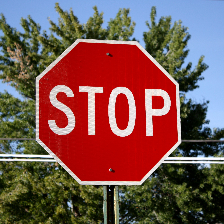
\includegraphics[width=0.2\linewidth]{../test_images/stop.png} &  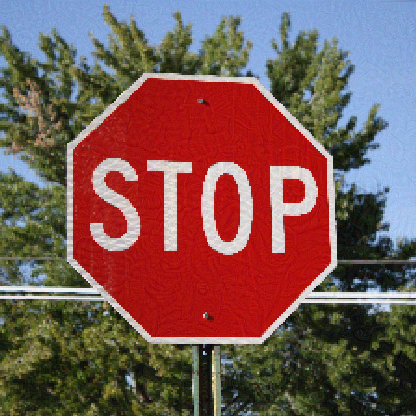
\includegraphics[width=0.2\linewidth]{../test_images/adversarial_out/stop.png} & 
        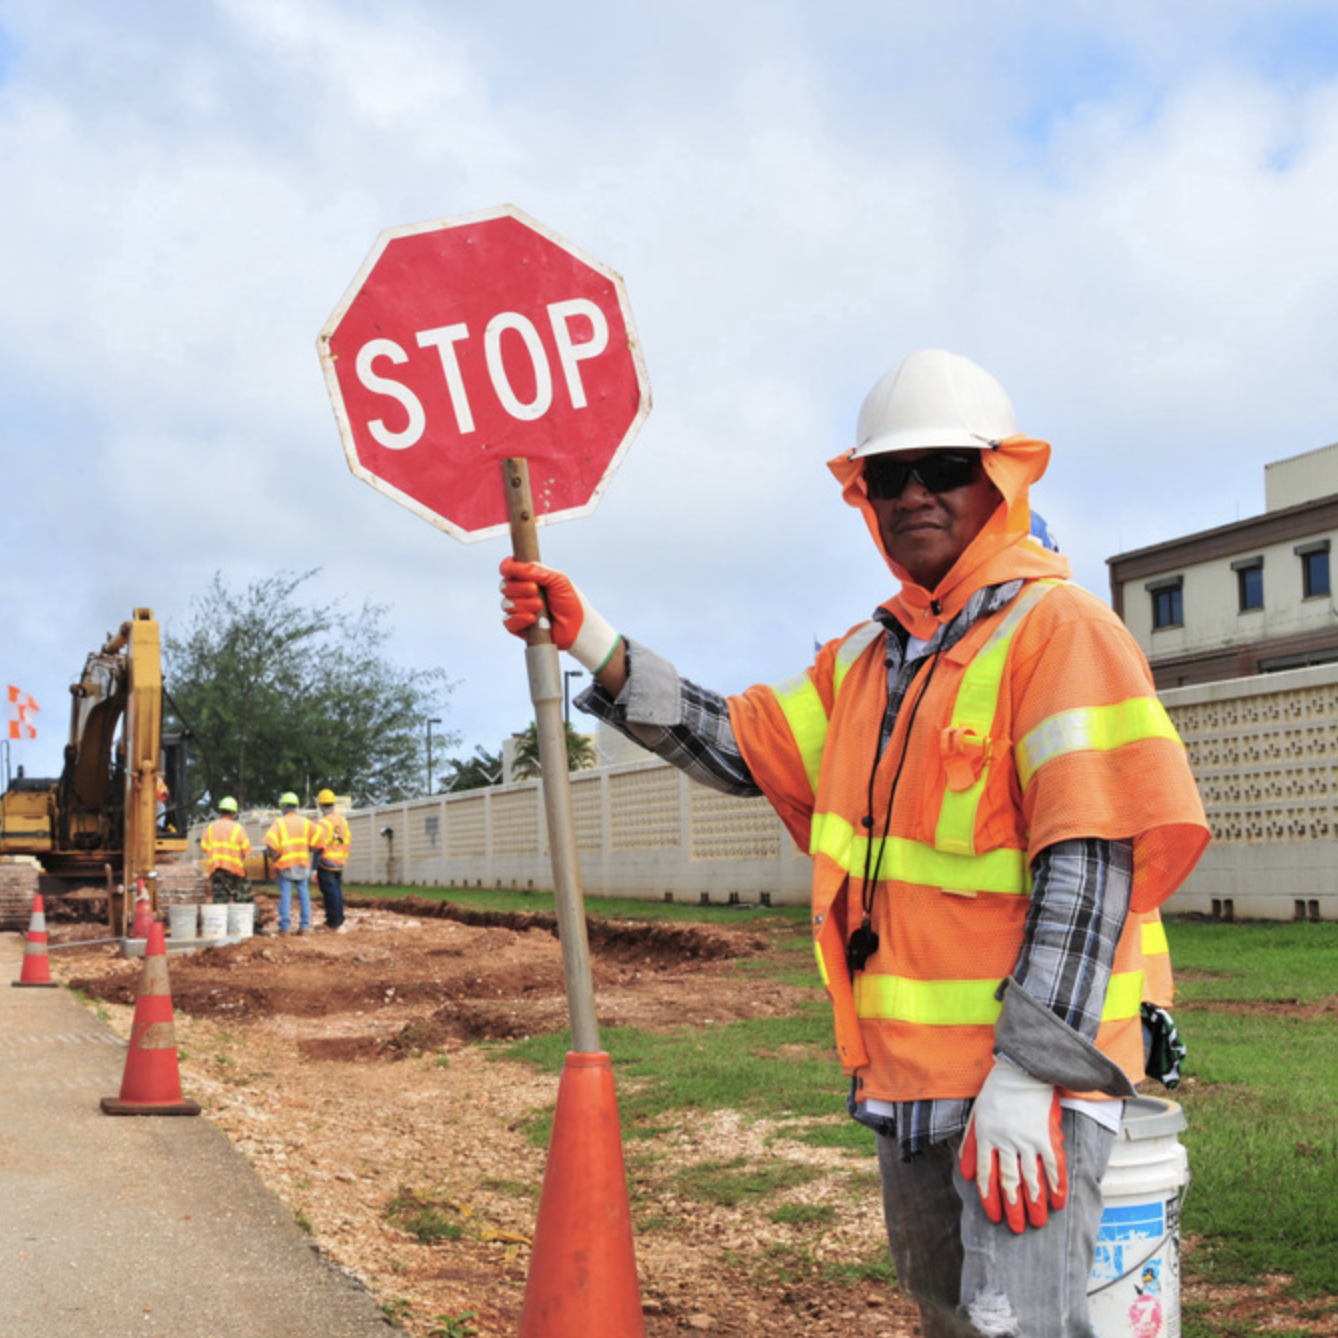
\includegraphics[width=0.2\linewidth]{../test_images/stop2.png} &  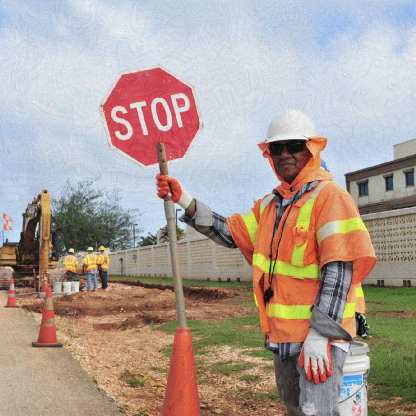
\includegraphics[width=0.2\linewidth]{../test_images/adversarial_out/stop2.png} \\

        \makecell[t]{YOLOv3 = 0.99987 \\ RCNN = 0.99987} & \makecell[t]{YOLOv3 = nothing \\ RCNN = 0.98742} & \makecell[t]{YOLOv3 = 0.99995 \\ RCNN = 0.99894} & \makecell[t]{YOLOv3 = nothing \\ RCNN = 0.99921} \\[1cm]

        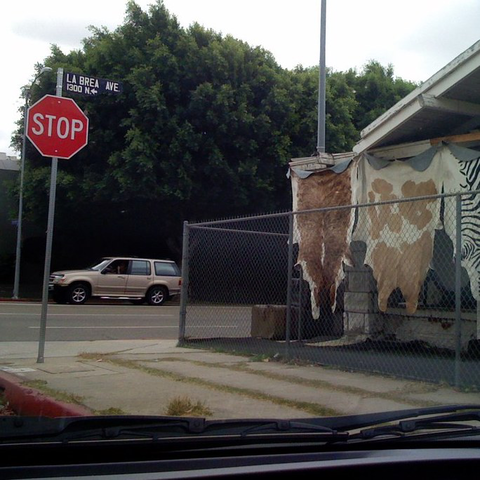
\includegraphics[width=0.2\linewidth]{../test_images/stop3.png} &  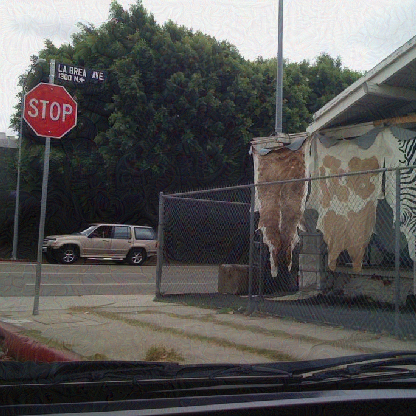
\includegraphics[width=0.2\linewidth]{../test_images/adversarial_out/stop3.png} & 
        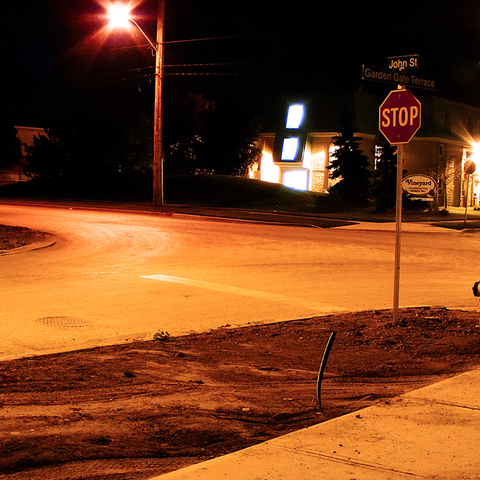
\includegraphics[width=0.2\linewidth]{../test_images/stop4.png} &  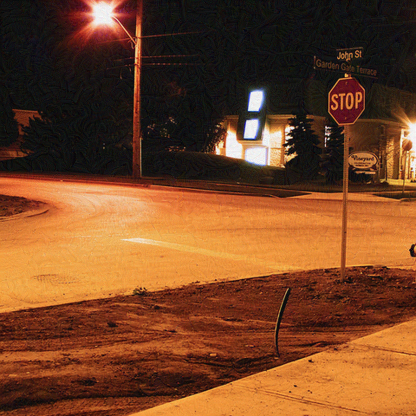
\includegraphics[width=0.2\linewidth]{../test_images/adversarial_out/stop4.png} \\

        \makecell[t]{YOLOv3 = 0.99971 \\ RCNN = 0.99839} & \makecell[t]{YOLOv3 = nothing \\ RCNN = 0.99855} & \makecell[t]{YOLOv3 = 0.99991 \\ RCNN = 0.99904} & \makecell[t]{YOLOv3 = nothing \\ RCNN = 0.99883} \\
    \end{tabular}
\caption{Adversarial Images for YOLOv3}
\label{fig:yoloadversarial}
\end{figure}

An experiment was run to determine the effectiveness of this attack across several different stop sign images. 11 images were used in total, where the stop signs were varying distances away from the camera. For all 11 images, this attack was able to create adversarial images that look very similar to their source images and were able to trick YOLOv3. However, this did not transfer to RCNN \cite{ren2016faster} which was able to easily detect all the stop signs in all of the images.

\section{Ensemble Adversarial Examples}

The LowKey adversarial attack \cite{cherepanova2021lowkey} on AWS Rekognition was successful by creating adversarial images that are able to fool multiple models at once. The technique is the same as the one used for adversarial examples against YOLOv3 \cite{redmon2018yolov3} except RCNN \cite{ren2016faster} was added in as well. The loss function to minimize is the confidence score of the bounding boxes predicted by both models. This loss is regularized by the Euclidean distance between the adversarial image and the original image as was done for producing the adversarial images for YOLOv3.

\begin{equation}
    \eta = \epsilon (\nabla_x ag(f_{\text{yolo}}(x)) + bg(f_{\text{rcnn}}(x) + c(x - \hat{x})^2))
\end{equation}

Where $\epsilon$ is the learning rate and $g$ is a function to extract the confidence scores of the bounding boxes from the output matrices of YOLOv3 and RCNN. $f_{\text{yolo}}$ is the YOLOv3 model and $f_{\text{rcnn}}$ is the Faster-RCNN model. $a$, $b$, and $c$ are scaling constants to make sure the individual network losses are of the same magnitude. This equation was run for 30 iterations of gradient descent to create adversarial images that can fool both networks. The results are visible in figure \ref{fig:yoloadversarial}, the confidence scores for the stop signs are listed beneath each of the images.

\begin{figure}[h]
\centering
    \begin{tabular}{c c@{\hskip 1cm} c c}
        original & adversarial & original & adversarial \\
        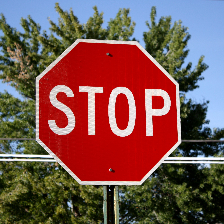
\includegraphics[width=0.2\linewidth]{../test_images/stop.png} &  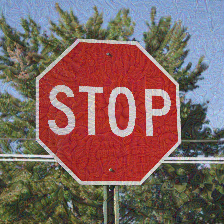
\includegraphics[width=0.2\linewidth]{../test_images/ensemble_adversarials/stop.png} & 
        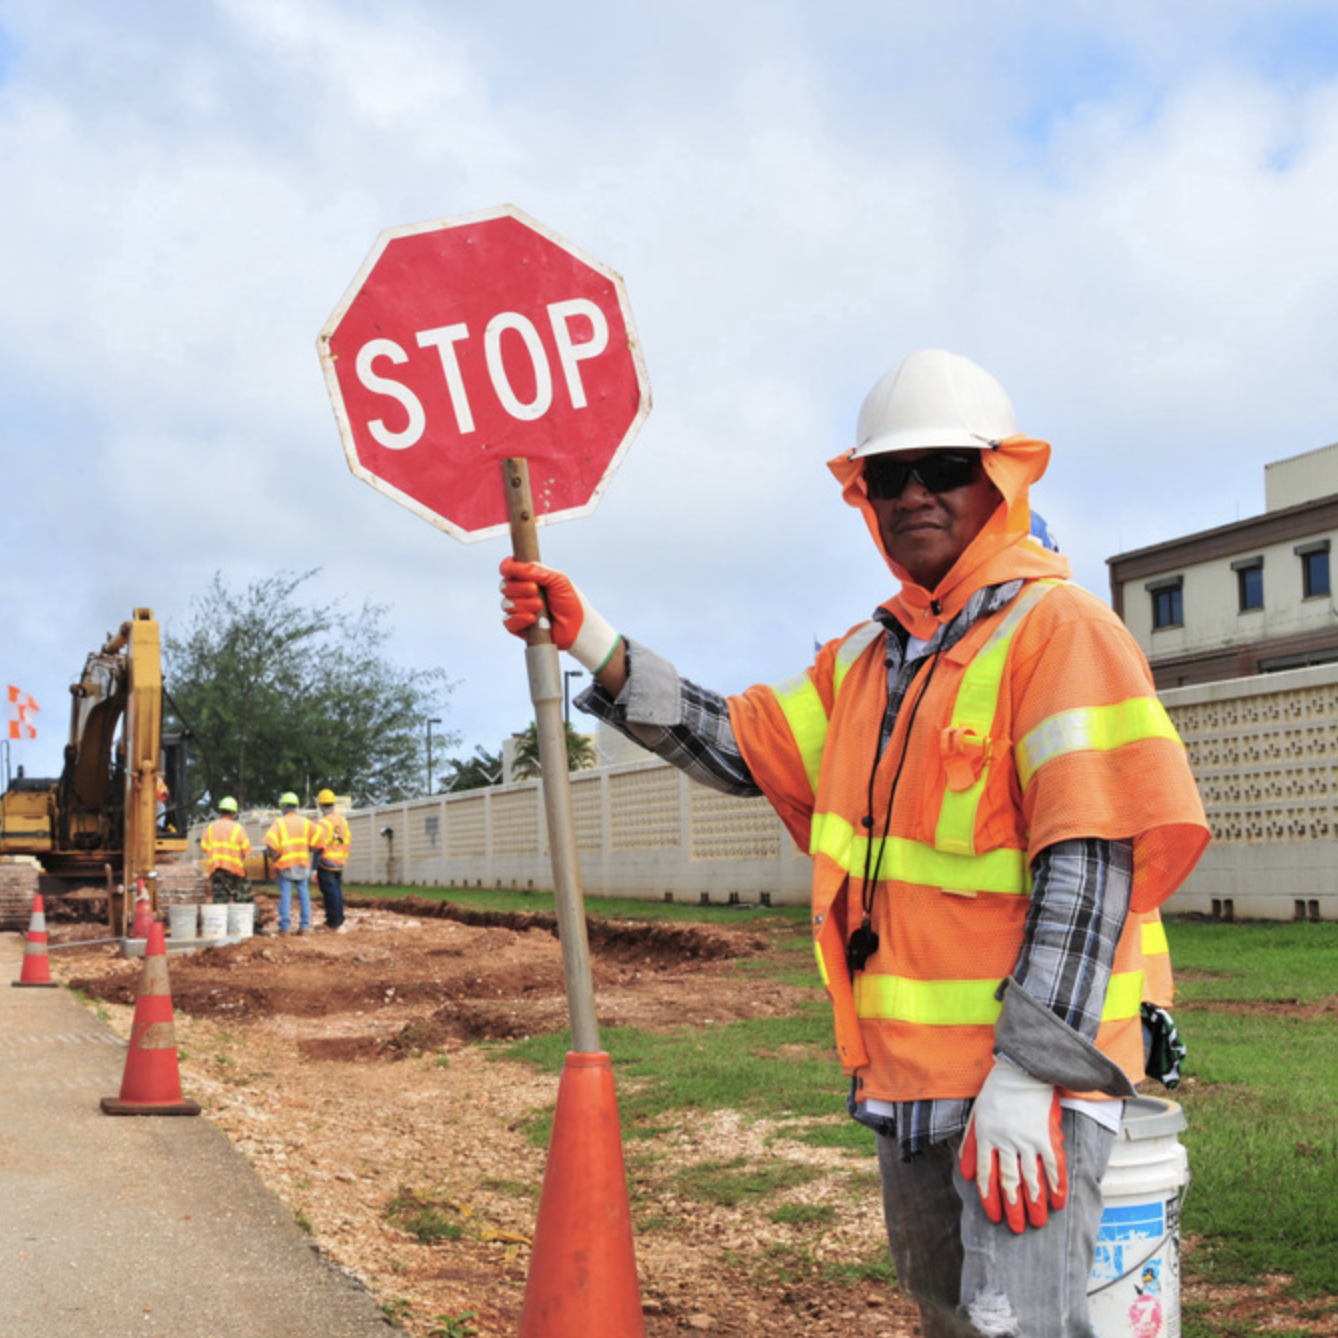
\includegraphics[width=0.2\linewidth]{../test_images/stop2.png} &  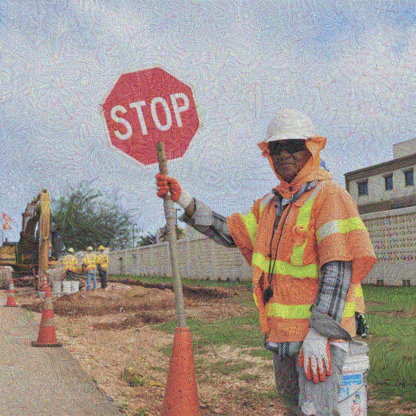
\includegraphics[width=0.2\linewidth]{../test_images/ensemble_adversarials/stop2.png} \\

        \makecell[t]{YOLOv3 = 0.99987 \\ RCNN = 0.99987} & \makecell[t]{YOLOv3 = nothing \\ RCNN = nothing} & \makecell[t]{YOLOv3 = 0.99995 \\ RCNN = 0.99894} & \makecell[t]{YOLOv3 = nothing \\ RCNN = nothing} \\[1cm]

        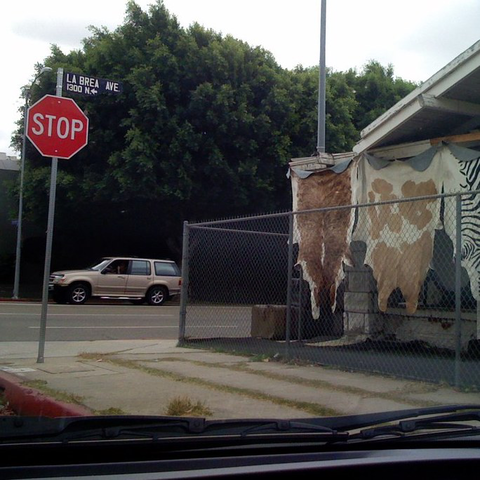
\includegraphics[width=0.2\linewidth]{../test_images/stop3.png} &  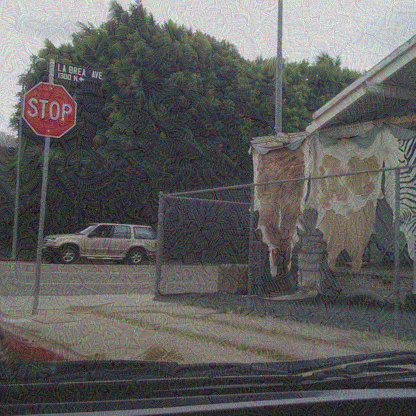
\includegraphics[width=0.2\linewidth]{../test_images/ensemble_adversarials/stop3.png} & 
        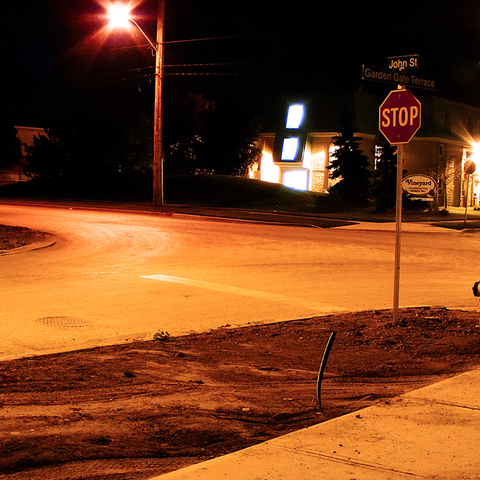
\includegraphics[width=0.2\linewidth]{../test_images/stop4.png} &  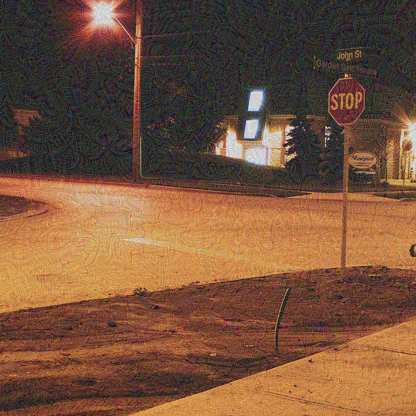
\includegraphics[width=0.2\linewidth]{../test_images/ensemble_adversarials/stop4.png} \\

        \makecell[t]{YOLOv3 = 0.99971 \\ RCNN = 0.99839} & \makecell[t]{YOLOv3 = nothing \\ RCNN = nothing} & \makecell[t]{YOLOv3 = 0.99991 \\ RCNN = 0.99904} & \makecell[t]{YOLOv3 = nothing \\ RCNN = 0.06873} \\
    \end{tabular}
\caption{Adversarial Images for YOLOv3 and FasterRCNN}
\label{fig:yoloadversarial}
\end{figure}

\section{Dispersion Reduction}
Dispersion reduction \cite{Lu_2020_CVPR} is a technique of creating adversarial images that are capable of fooling black box object detectors. A known source model, like VGG-16 \cite{simonyan2015deep}, is used to create the adversarial images that can hopefully fool any object detector network without ever having access to it.

Each layer of the known image classifier  VGG-16 produces a feature map. The level of abstraction of the features increases the deeper in the network that they're produced. The early layers extract simple features like edges and shapes, while the later layers extract higher level features like a dog's nose. \cite{olah2017feature}

The dispersion reduction attack aims to adjust the input image so that the feature map produced from it doesn't contain the features that are visibly present to a human in the image. This attack works by reducing the standard deviation of the target feature map. The source network is evaluated up until the layer that produces the target feature map, then the standard deviation of it is calculated and the derivative of this value is computed with respect to the input image. The sign of the resulting gradient is then added back to the input image to reduce the standard deviation of its feature map. The equation below describes how the adversarial adjustment is calculated. The input image is $x$, the learning rate is $\epsilon$ and $f_{\text{fm}}$ is VGG-16 evaluated up until the target feature map, fm.

\begin{equation}
    \eta = - \epsilon * \text{sign}(\nabla_x \text{std}(f_{\text{fm}}(x)))
\end{equation}

Experiments were run to determine the effectiveness of this attack with hiding stop signs from object detectors. For this experiment the output of the 12th layer of VGG-16 was used as the feature map to reduce, which is a tensor of size (256, 120, 120). The original image was updated using the above equation for 25 and 50 iterations of gradient descent with $\epsilon = 2$ and the results are shown in figures \ref{fig:drskier}, \ref{fig:stop1} and \ref{fig:stop3}.


\begin{figure}[h]
\centering
    \begin{tabular}{c c c}
        original & 25 iterations & 50 iterations \\
        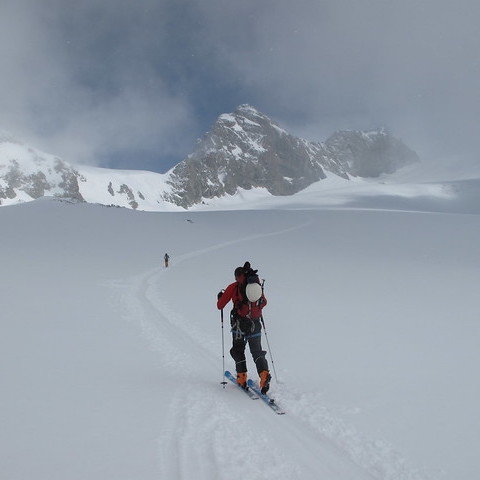
\includegraphics[width=0.3\linewidth]{../test_images/skiers.jpg} & 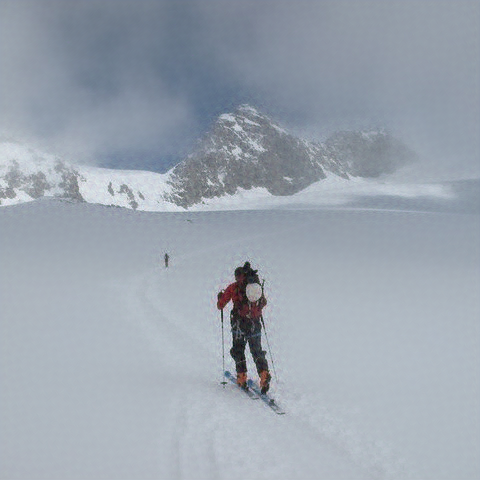
\includegraphics[width=0.3\linewidth]{../test_images/dispersion_reduced/skiers25.png} & 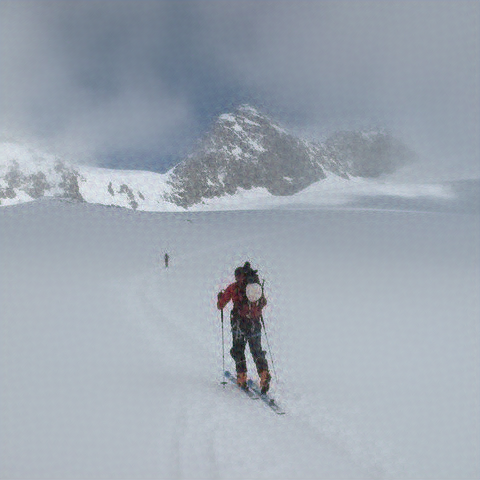
\includegraphics[width=0.3\linewidth]{../test_images/dispersion_reduced/skiers50.png} \\

        \makecell[t]{\textbf{YOLOv3} \\ person 0.99993 \\ skis 0.99864 \\ person 0.99809 \\ \\ \textbf{RCNN} \\ person 0.99927 \\ skis 0.99780 \\ person 0.98474 \\ backpack 0.82482} & \makecell[t]{\textbf{YOLOv3} \\ person 0.99994 \\ \\ \textbf{RCNN} \\ person 0.99928 \\ skis 0.99679 \\ person 0.93090 \\ backpack 0.71321 } & \makecell[t]{\textbf{YOLOv3} \\ person 0.99992 \\ \\ \textbf{RCNN} \\ person 0.99919 \\ skis 0.99537 \\ person 0.86015 \\ backpack 0.62698} \\[4.5cm]
    \end{tabular}
\caption{Dispersion Reduction on Skier}
\label{fig:drskier}
\end{figure}

\begin{figure}[h]
\centering
    \begin{tabular}{c c c}
        \includegraphics[width=0.3\linewidth]{../test_images/stop.png} & \includegraphics[width=0.3\linewidth]{../test_images/dispersion_reduced/stop25.png} & \includegraphics[width=0.3\linewidth]{../test_images/dispersion_reduced/stop50.png} \\

        \makecell[t]{\textbf{YOLOv3} \\ stop sign 0.99987 \\ \\ \textbf{RCNN} \\ stop sign 0.99987} & \makecell[t]{\textbf{YOLOv3} \\ stop sign 0.99985 \\ \\ \textbf{RCNN} \\ stop sign 0.99976} & \makecell[t]{\textbf{YOLOv3} \\ stop sign 0.99985 \\ \\ \textbf{RCNN} \\ stop sign 0.99662}
\end{tabular}
\caption{Dispersion Reduction on Big Stop Sign}
\label{fig:stop1}
\end{figure}

\begin{figure}[h]
\centering
    \begin{tabular}{c c c}
        \includegraphics[width=0.3\linewidth]{../test_images/stop3.png} & \includegraphics[width=0.3\linewidth]{../test_images/dispersion_reduced/stop3_25.png} & \includegraphics[width=0.3\linewidth]{../test_images/dispersion_reduced/stop3_50.png} \\

        \makecell[t]{\textbf{YOLOv3} \\ stop sign 0.99971 \\ car 0.99317 \\ \\ \textbf{RCNN} \\ stop sign 0.99839 \\ car 0.91922 \\} & \makecell[t]{\textbf{YOLOv3} \\ stop sign 0.99974 \\ car 0.97653 \\ \\ \textbf{RCNN} \\ stop sign 0.99884 \\ car 0.90228} & \makecell[t]{\textbf{YOLOv3} \\ stop sign 0.99975 \\ car 0.97283 \\ \\ \textbf{RCNN} \\ stop sign 0.99880 \\ car 0.95387}
\end{tabular}
\caption{Dispersion Reduction on Small Stop Sign}
\label{fig:stop3}
\end{figure}

This attack seems to work for hiding objects in the image that are small or less pronounced like the skis in the first image. Even after just 25 iterations YOLOv3 was unable to detect the skis. However, this attack had less of an effect on RCNN with it only reducing the confidence scores of the person in the distance and the backpack. For hiding stop signs this attack didn't work at all. For both YOLOv3 and RCNN the attack hardly even changed the confidence scores for either stop sign image. This is likely due to the fact that stop signs have a unique shape, color and font that is unlike the other object classes so the model is unlikely to confuse it with anything else. In addition stop signs are designed to be easy to see and stand out a lot against the background unlike the skis in the first image.

\clearpage
\bibliographystyle{unsrt}
\bibliography{references}

\end{document}